\chapter{Greedy Algorithms}
\chapterepigraph{A greedy algorithm commits to the choice that looks best
right now and never looks back. That is only safe when you can
\emph{prove} that some optimal solution agrees with your choice. In a
contest the proof is usually two lines long --- but those two lines are the
difference between an Accepted and a Wrong Answer on test 37.}

\section{Theory and Must-Know Patterns}
\label{sec:greedy-theory}

A greedy algorithm builds a solution one decision at a time, always taking
the locally best option by some rule. Three questions decide whether a
greedy is correct:
\begin{enumerate}
  \item \textbf{What is the rule?} (``earliest end time first'', ``smallest
        element first'', ``largest coin that fits'', \dots)
  \item \textbf{Why does some optimal solution follow the rule?} (the
        proof --- usually an exchange argument)
  \item \textbf{How do I apply the rule fast?} (sorting, a heap, a
        multiset, two pointers)
\end{enumerate}

\subsection*{Proof technique 1: the exchange argument}

Take any optimal solution $O$ that disagrees with the greedy choice $g$.
Modify $O$ by swapping in $g$ and show the result is still valid and no
worse. Repeating the swap turns $O$ into the greedy solution without ever
losing value, so greedy is optimal.

\begin{center}
\begin{tikzpicture}[x=0.9cm,y=0.75cm,>=Stealth]
  \draw[->] (0,0) -- (12.5,0) node[right] {\small time};
  % optimal row
  \node[left] at (0,1.6) {\small optimal $O$};
  \draw[fill=blue!15] (2.2,1.3) rectangle (6.0,1.9) node[midway] {\small $o_1$};
  \draw[fill=blue!15] (6.5,1.3) rectangle (9.0,1.9) node[midway] {\small $o_2$};
  \draw[fill=blue!15] (9.5,1.3) rectangle (12.0,1.9) node[midway] {\small $o_3$};
  % greedy row
  \node[left] at (0,0.6) {\small greedy};
  \draw[fill=orange!25] (1.0,0.3) rectangle (4.5,0.9) node[midway] {\small $g$ (ends first)};
  \draw[dashed] (4.5,0) -- (4.5,2.1);
  \draw[dashed] (6.0,0) -- (6.0,2.1);
  \draw[decorate,decoration={brace,amplitude=4pt,mirror}] (4.5,-0.15) -- (6.0,-0.15)
     node[midway,below=4pt] {\small $e(g)\le e(o_1)$};
\end{tikzpicture}
\end{center}

\noindent In interval scheduling (Section~\ref{sec:g-movie}) the interval
$g$ with the earliest end time finishes no later than $o_1$, so replacing
$o_1$ by $g$ cannot collide with $o_2, o_3, \dots$ --- the solution keeps
the same size.

\subsection*{Proof technique 2: greedy stays ahead}

Show by induction that after every step the greedy partial solution is at
least as good as any other partial solution by some measure (``has watched
at least as many movies and is free at least as early''). Then at the end it
is at least as good as the optimum.

\subsection*{Proof technique 3: a matching lower bound}

Find a quantity every solution must pay (``each non-survivor unit must be
removed'', ``someone must miss problem $i$ in $n-a_i$ places'') and show
the greedy pays exactly that. Several prelim problems in this chapter are
solved this way: the formula is a lower bound, and the greedy construction
achieves it.

\subsection*{The ICPC greedy toolkit}

\begin{center}
\renewcommand{\arraystretch}{1.25}
\begin{tabular}{p{4.2cm}p{5.2cm}p{4.3cm}}
\toprule
\textbf{Pattern} & \textbf{Typical rule} & \textbf{Problems here}\\
\midrule
Sort + scan & process in sorted order, keep a running value & Movie Festival, Tasks and Deadlines, Wormhole, Missing Coin Sum\\
Median / extremes & optimum sits at a median or at max/min & Stick Lengths, Task Scheduling, Reading Books\\
Multiset ``best fit'' & take the closest item $\le$ or $>$ a key & Concert Tickets, Towers, Traffic Lights\\
Heap of resources & reuse the resource that frees earliest & Room Allocation, Coins (top-$X$ sums)\\
Sweep line / difference array & $+1$ at start, $-1$ after end & Restaurant Customers, Game of Robots\\
Two pointers & window never needs to move left & Playlist, Cracker shops\\
Binary search on the answer & ``can we finish by time $T$?'' is monotone & Factory Machines\\
Huffman / merge smallest & repeatedly combine the two cheapest & Break, Merge and Sort\\
Counting argument & answer = forced lower bound & Good Contest, Boss Fight, Reduction Game, Always Changing\\
Parity invariant & an operation preserves parity of something & Tatar TV Show\\
\bottomrule
\end{tabular}
\end{center}

\begin{takeawaybox}[Contest Checklist Before Submitting a Greedy]
\begin{enumerate}
  \item Write the exchange (or lower-bound) argument in one sentence. If
        you cannot, brute-force small cases first.
  \item Check ties: does the sort key need a secondary key?
  \item Check overflow: sums of $2\cdot10^5$ values up to $10^9$ need
        \texttt{long long}.
  \item Check the empty / single-element / all-equal cases.
\end{enumerate}
\end{takeawaybox}

\noindent Problems are ordered roughly from easy to hard. Every C++ listing
in this chapter is the exact file in \texttt{icpc-training/greedy/}, and
every one of them passes the official samples plus randomised stress tests
against an exhaustive brute force (\texttt{tests/}).

\newpage

\section{Task Scheduling Problem}
\label{sec:g-task-scheduling}
\problemlink{https://atcoder.jp/contests/abc103/tasks/abc103_a}{AtCoder ABC103 A}
\source{AtCoder ABC103 A (Notion: Greedy)}{Easy}

\problemstatement{There are three tasks with values $A_1,A_2,A_3$
($1\le A_i\le 100$). The first task you complete costs $0$; completing task
$j$ right after task $i$ costs $|A_j-A_i|$. Find the minimum total cost to
complete all three tasks.}

\begin{patternbox}
``Visit points on a line, pay the distance between consecutive visits'' ---
the cost of any route is at least the length of the segment it covers.
\end{patternbox}

\subsection*{Approach and intuition}

Put the three values on a number line. Any order of visiting them must
travel from the smallest to the largest value at some point, so every order
costs at least $\max A-\min A$. Visiting them in sorted order walks
monotonically from $\min$ to $\max$ and costs exactly that amount.

\begin{ideabox}[Why It Is Optimal]
\emph{Lower bound:} the route touches both $\min A$ and $\max A$; by the
triangle inequality the total path length between those two visits is at
least $\max A-\min A$. \emph{Achievability:} sorted order has cost
$(A_{(2)}-A_{(1)})+(A_{(3)}-A_{(2)})=A_{(3)}-A_{(1)}$.
\end{ideabox}

\subsection*{Algorithm}
\begin{algorithmic}[1]
\State read $A_1,A_2,A_3$
\State \Return $\max(A_1,A_2,A_3)-\min(A_1,A_2,A_3)$
\end{algorithmic}

\dryrun{$A=(1,6,3)$: sorted $1,3,6$, cost $2+3=5=6-1$. \checkmark}

\subsection*{C++17 implementation}
\cppfile{greedy/01_task_scheduling.cpp}

\begin{complexitybox}
\textbf{Time:} $O(1)$. \textbf{Space:} $O(1)$.
\end{complexitybox}

\begin{pitfallbox}
\begin{itemize}
  \item All equal values ($100\ 100\ 100$) give $0$ --- the formula
        handles it.
  \item The same idea generalises to $n$ points: answer $\max-\min$, not a
        sum of sorted gaps you must compute one by one.
\end{itemize}
\end{pitfallbox}

\section{Good Contest}
\label{sec:g-good-contest}
\problemlink{https://codeforces.com/problemset/problem/2266/A}{Codeforces 2266A}
\source{Codeforces 2266A (Notion: Greedy, 800)}{Easy}

\problemstatement{A contest has three problems and $n$ participants
($1\le n\le 9$). Problem $i$ was solved by exactly $a_i$ participants
($0\le a_i\le n$). A participant is \emph{weak} if they did not solve all
three problems. Over all scoreboards consistent with $a$, find the minimum
possible number of weak participants. ($t\le 3000$ test cases.)}

\begin{patternbox}
``Minimum number of people who miss \emph{something}'' --- overlap the
misses as much as possible. The answer is a lower bound that one
construction meets.
\end{patternbox}

\subsection*{Approach and intuition}

Problem $i$ is \emph{missed} by $n-a_i$ participants, and each of them is
weak. Hence at least $\max_i(n-a_i)$ participants are weak. To achieve this,
number the participants $1..n$ and let the misses of every problem fall on
the \emph{first} participants: problem $i$ is missed by participants
$1,\dots,n-a_i$. Then exactly participants $1,\dots,\max_i(n-a_i)$ miss
something.

\begin{ideabox}[Lower Bound Meets Construction]
\[
  \text{answer} = \max(n-a_1,\;n-a_2,\;n-a_3).
\]
\end{ideabox}

\subsection*{Algorithm}
\begin{algorithmic}[1]
\For{each test case}
  \State \textbf{print} $\max(n-a_1,n-a_2,n-a_3)$
\EndFor
\end{algorithmic}

\dryrun{$n=6$, $a=(4,3,2)$: misses are $2,3,4$; stacking them on
participants $1..4$ gives $4$ weak participants. $n=5$, $a=(0,5,5)$: all
$5$ miss problem~1, answer $5$. \checkmark}

\subsection*{C++17 implementation}
\cppfile{greedy/02_good_contest.cpp}

\begin{complexitybox}
\textbf{Time:} $O(1)$ per test. \textbf{Space:} $O(1)$.
\end{complexitybox}

\begin{pitfallbox}
\begin{itemize}
  \item Do \emph{not} add the misses: $\sum(n-a_i)$ counts a participant
        who misses two problems twice.
  \item $a_i=n$ for all $i$ gives $0$.
\end{itemize}
\end{pitfallbox}

\section{Boss Fight}
\label{sec:g-boss-fight}
\problemlink{https://codeforces.com/problemset/problem/2252/A}{Codeforces 2252A}
\source{Codeforces 2252A (Notion: Greedy, 800)}{Easy}

\problemstatement{You have $n\le 50$ spell cards; card $i$ deals $a_i$
damage ($1\le a_i\le1000$). You may play them in any order. If you ever play
two cards of \emph{equal} damage consecutively, a shield activates: the
triggering card still deals its damage, but every later card deals $0$.
Find the maximum total damage.}

\begin{patternbox}
``Arrange items so that no two equal items are adjacent'' is possible iff the
most frequent value $v$ with frequency $f$ satisfies $f\le (n-f)+1$. When it
fails, the dominant value is the only obstacle.
\end{patternbox}

\subsection*{Approach and intuition}

Let $v$ be the most frequent damage value, $f$ its frequency, $r=n-f$ the
number of other cards and $R$ their total damage.

\begin{itemize}
  \item If $f\le r+1$ we can interleave (\,$v\,x\,v\,x\dots$) so no two equal
        cards touch: every card counts, answer $=\sum a_i$.
  \item Otherwise play $v,x_1,v,x_2,\dots,x_r,v$ (all $r$ others and $r+1$
        copies of $v$, no equal neighbours) and then one more $v$ as the
        trigger. Damage $=R+(r+2)v$.
\end{itemize}

\begin{ideabox}[Why $r+2$ Copies Is the Maximum]
Before the trigger, the played cards have no equal neighbours, so among
them at most (number of other cards) $+1\le r+1$ are copies of $v$. The
trigger adds one more. No other card is ever lost, so the construction is
optimal:
\[
\text{answer}=\begin{cases}\sum a_i & f\le r+1\\ R+\min(f,r+2)\cdot v & \text{otherwise.}\end{cases}
\]
(If a different value triggered the shield we would only lose more copies
of $v$.)
\end{ideabox}

\subsection*{Algorithm}
\begin{algorithmic}[1]
\State count frequencies; let $v$ be a value of maximum frequency $f$
\State $r\gets n-f$, $R\gets \sum a - f\cdot v$
\If{$f\le r+1$} \Return $\sum a$
\Else \ \Return $R+\min(f,r+2)\cdot v$
\EndIf
\end{algorithmic}

\dryrun{$a=[10,5,10,10]$: $v=10$, $f=3$, $r=1$, $3>2$, so answer
$5+3\cdot10=35$ (order $10,5,10,10$). $a=[7^6]$: $r=0$, answer
$0+2\cdot7=14$. \checkmark}

\subsection*{C++17 implementation}
\cppfile{greedy/03_boss_fight.cpp}

\begin{complexitybox}
\textbf{Time:} $O(n\log n)$ per test (map of frequencies).
\textbf{Space:} $O(n)$.
\end{complexitybox}

\begin{pitfallbox}
\begin{itemize}
  \item $n=1$: $f=1\le 0+1$, the single card counts.
  \item The trigger card \emph{does} deal damage --- forgetting it gives
        $R+(r+1)v$.
\end{itemize}
\end{pitfallbox}

\section{Flee to Shelter}
\label{sec:g-flee}
\problemlink{https://github.com/m-e-r-l-i-n/icpc-india/blob/main/src/2013amritapuri_online.pdf}{Contest PDF (Amritapuri 2013 Online)}
\source{ICPC 2013--14 Amritapuri Online Round (PYQ)}{Easy}

\problemstatement{Dr.~Stone is at the shuttle and must bring $N$
instruments from the telescope to the shuttle. She can carry at most $M$
instruments per trip, and a one-way walk between the two takes $T$ minutes.
Find the minimum total time ($1\le N,M,T\le100$, up to $1000$ tests).}

\begin{patternbox}
Trips of fixed cost with a capacity limit: always fill the capacity.
Number of trips $=\lceil N/M\rceil$.
\end{patternbox}

\subsection*{Approach and intuition}

Every trip consists of walking to the telescope ($T$) and back loaded
($T$). A trip carries at most $M$ instruments, so at least $\lceil
N/M\rceil$ trips are needed; carrying $M$ each time (and the remainder last)
achieves that. She starts at the shuttle and must end there, so the answer
is
\[
  2T\left\lceil \frac{N}{M}\right\rceil .
\]

\subsection*{Algorithm}
\begin{algorithmic}[1]
\State $trips\gets (N+M-1)\ \mathrm{div}\ M$ \Comment{integer ceiling}
\State \Return $2\cdot trips\cdot T$
\end{algorithmic}

\dryrun{$N=3$, $M=2$, $T=10$: $\lceil3/2\rceil=2$ trips, $2\cdot2\cdot10=40$.
\checkmark}

\subsection*{C++17 implementation}
\cppfile{greedy/04_flee_to_shelter.cpp}

\begin{complexitybox}
\textbf{Time:} $O(1)$ per test. \textbf{Space:} $O(1)$.
\end{complexitybox}

\begin{pitfallbox}
\begin{itemize}
  \item Use integer ceiling $(N+M-1)/M$; floating \texttt{ceil} is
        unnecessary.
  \item She starts at the \emph{shuttle}, so even the first trip costs
        $2T$ (walk out, walk back).
\end{itemize}
\end{pitfallbox}

\section{Ordering Teams}
\label{sec:g-ordering-teams}
\source{ICPC 2017--18 Online Preliminary, Kharagpur (PYQ, ORDTEAMS)}{Easy}

\problemstatement{Three team members have scores $(s_1,s_2,s_3)$ in three
skills. Person $x$ is \emph{better} than $y$ if $x$ scores no less than $y$ in
every skill and strictly more in at least one. Decide whether the three can
be ordered so that each person is strictly better than the previous one.}

\begin{patternbox}
A dominance chain is increasing in \emph{every} coordinate, hence in the
coordinate sum. Sorting by the sum fixes the only possible order.
\end{patternbox}

\subsection*{Approach and intuition}

If $x$ is better than $y$ then $\text{sum}(x)>\text{sum}(y)$ (no coordinate
drops, one rises). So in any valid chain the sums strictly increase, which
means the chain must be the order by increasing sum. Sort the three people by
their sum and check the two consecutive relations. With ties in the sum, the
two tied people cannot be ordered, and the check fails automatically.

\subsection*{Algorithm}
\begin{algorithmic}[1]
\State sort the three people by $s_1+s_2+s_3$
\State \Return \textsc{Better}$(p_2,p_1)$ \textbf{and} \textsc{Better}$(p_3,p_2)$
\end{algorithmic}

\dryrun{Case 1: sums $6,9,10$; $(2,3,4)$ beats $(1,2,3)$ and $(2,3,5)$ beats
$(2,3,4)$ $\Rightarrow$ yes. Case 2: $(2,3,4)$ appears twice, not strictly
better $\Rightarrow$ no. \checkmark}

\subsection*{C++17 implementation}
\cppfile{greedy/05_ordering_teams.cpp}

\begin{complexitybox}
\textbf{Time:} $O(1)$ per test. \textbf{Space:} $O(1)$.
\end{complexitybox}

\begin{pitfallbox}
\begin{itemize}
  \item ``Better'' needs a \emph{strict} improvement somewhere: identical
        people cannot be chained.
  \item Output is lowercase \texttt{yes}/\texttt{no}.
\end{itemize}
\end{pitfallbox}

\section{Stick Lengths}
\label{sec:g-stick-lengths}
\problemlink{https://cses.fi/problemset/task/1074}{CSES 1074}
\source{CSES 1074 (Notion: Greedy)}{Easy}

\problemstatement{There are $n\le2\cdot10^5$ sticks of lengths $p_i\le10^9$.
Changing a stick's length by $x$ costs $x$. Make all sticks equal with minimum
total cost.}

\begin{patternbox}
Minimise $\sum|p_i-x|$ over $x$: the answer is at a \textbf{median}.
(Minimising $\sum(p_i-x)^2$ would give the mean instead.)
\end{patternbox}

\subsection*{Approach and intuition}

Let $c(x)=\sum_i |p_i-x|$. Moving $x$ one unit to the right changes the cost
by (number of sticks $\le x$) $-$ (number of sticks $>x$). While fewer than
half of the sticks are to the left, moving right helps; once at least half are
to the left, it hurts. The turning point is the median.

\begin{center}
\begin{tikzpicture}[x=0.7cm,y=0.45cm]
  \draw[->] (0,0) -- (11,0) node[right] {\small $x$};
  \draw[->] (0,0) -- (0,6) node[above] {\small $c(x)$};
  \draw[thick,blue] (0.5,5.6) -- (1,4.6) -- (2,3.1) -- (3,2.1) -- (5,1.5) -- (7,2.1) -- (9,4.1) -- (10.5,5.6);
  \foreach \x/\l in {1/1,2/2,3/2,5/3,9/5} \fill (\x,0) circle (2pt);
  \node[below] at (3,0) {\small median};
  \draw[dashed] (3,0) -- (3,2.1);
\end{tikzpicture}
\end{center}

\noindent $c$ is convex and piecewise linear with slope
$\#\{p_i<x\}-\#\{p_i>x\}$; it is minimal where the slope changes sign.

\subsection*{Algorithm}
\begin{algorithmic}[1]
\State $m\gets$ the element of rank $\lfloor n/2\rfloor$ (\texttt{nth\_element})
\State \Return $\sum_i |p_i-m|$
\end{algorithmic}

\dryrun{$p=[2,3,1,5,2]$, sorted $1,2,2,3,5$, median $2$. Cost
$0+1+1+3+0=5$. \checkmark}

\subsection*{C++17 implementation}
\cppfile{greedy/06_stick_lengths.cpp}

\begin{complexitybox}
\textbf{Time:} $O(n)$ expected (\texttt{nth\_element}). \textbf{Space:} $O(n)$.
\end{complexitybox}

\begin{pitfallbox}
\begin{itemize}
  \item The cost can reach $2\cdot10^5\cdot10^9=2\cdot10^{14}$: use
        \texttt{long long}.
  \item For even $n$ any value between the two middle elements is optimal;
        picking either middle element is fine.
\end{itemize}
\end{pitfallbox}

\section{Movie Festival}
\label{sec:g-movie}
\problemlink{https://cses.fi/problemset/task/1629}{CSES 1629}
\source{CSES 1629 (Notion: Greedy)}{Easy}

\problemstatement{$n\le2\cdot10^5$ movies are shown; movie $i$ runs from
$a_i$ to $b_i$ ($a_i<b_i\le10^9$). What is the maximum number of movies you
can watch completely? (A movie may start exactly when the previous ends.)}

\begin{patternbox}
Interval scheduling / activity selection: \textbf{pick the interval that
ends first}, discard everything overlapping it, repeat.
\end{patternbox}

\subsection*{Approach and intuition}

Sort by end time. Keep \texttt{freeAt}, the end of the last chosen movie.
Scan the movies; take a movie whenever it starts at or after
\texttt{freeAt}.

\begin{ideabox}[Exchange Argument]
Let $g$ be the movie that ends first and $O$ an optimal schedule whose first
movie is $o_1\ne g$. Since $b_g\le b_{o_1}$, replacing $o_1$ by $g$ keeps $O$
feasible (everything after $o_1$ starts at or after $b_{o_1}\ge b_g$) and of
the same size. So some optimal schedule starts with $g$; recurse on the
movies starting after $b_g$. (See the picture in
Section~\ref{sec:greedy-theory}.)
\end{ideabox}

\subsection*{Algorithm}
\begin{algorithmic}[1]
\State sort movies by end time
\State $cnt\gets0$, $freeAt\gets0$
\For{each movie $(a,b)$ in that order}
  \If{$a\ge freeAt$} \State $cnt\gets cnt+1$, $freeAt\gets b$ \EndIf
\EndFor
\State \Return $cnt$
\end{algorithmic}

\dryrun{Movies $(3,5),(4,9),(5,8)$; by end: $(3,5),(5,8),(4,9)$. Take
$(3,5)$; $(5,8)$ starts at $5\ge5$, take; $(4,9)$ starts at $4<8$, skip.
Answer $2$. \checkmark}

\subsection*{C++17 implementation}
\cppfile{greedy/07_movie_festival.cpp}

\begin{complexitybox}
\textbf{Time:} $O(n\log n)$. \textbf{Space:} $O(n)$.
\end{complexitybox}

\begin{pitfallbox}
\begin{itemize}
  \item Sorting by \emph{start} time or by \emph{length} is wrong
        (a long early movie, or a short movie overlapping two others).
  \item Use $a\ge freeAt$, not $>$: back-to-back movies are allowed.
\end{itemize}
\end{pitfallbox}

\section{Restaurant Customers}
\label{sec:g-restaurant}
\source{CSES 1619 (Notion: Greedy)}{Easy}

\problemstatement{Customer $i$ is in the restaurant from time $a_i$ to $b_i$
($1\le a_i<b_i\le10^9$, all $2n$ times distinct, $n\le2\cdot10^5$). Find the
maximum number of customers present at the same time.}

\begin{patternbox}
``Maximum overlap of intervals'' $\Rightarrow$ \textbf{sweep line}: an
arrival is a $+1$ event, a departure a $-1$ event; the answer is the maximum
prefix sum in time order.
\end{patternbox}

\subsection*{Approach and intuition}

The number of people present only changes at event times. Sorting the $2n$
events and accumulating $\pm1$ reproduces the head count at every moment; its
maximum is the answer. Because times are distinct we never have to decide
whether a departure and an arrival at the same instant overlap.

\subsection*{Algorithm}
\begin{algorithmic}[1]
\State events $\gets \{(a_i,+1),(b_i,-1)\}$, sort by time
\State $cur\gets0$, $best\gets0$
\For{each event $(t,d)$} \State $cur\gets cur+d$, $best\gets\max(best,cur)$ \EndFor
\State \Return $best$
\end{algorithmic}

\dryrun{Intervals $(5,8),(2,4),(3,9)$: events $2^{+},3^{+},4^{-},5^{+},8^{-},9^{-}$,
counts $1,2,1,2,1,0$. Maximum $2$. \checkmark}

\subsection*{C++17 implementation}
\cppfile{greedy/08_restaurant_customers.cpp}

\begin{complexitybox}
\textbf{Time:} $O(n\log n)$. \textbf{Space:} $O(n)$.
\end{complexitybox}

\begin{pitfallbox}
\begin{itemize}
  \item If times could coincide you must decide the tie order (process
        $-1$ before $+1$ for half-open intervals). Here they are distinct.
  \item Coordinates up to $10^9$: never allocate an array indexed by time.
\end{itemize}
\end{pitfallbox}

\section{Tasks and Deadlines}
\label{sec:g-tasks-deadlines}
\source{CSES 1630 (Notion: Greedy)}{Easy}

\problemstatement{You must process all $n\le2\cdot10^5$ tasks one after
another starting at time $0$. Task $i$ has duration $a_i$ and deadline $d_i$;
finishing it at time $f_i$ earns $d_i-f_i$ (possibly negative). Maximise the
total reward.}

\begin{patternbox}
The objective splits into a fixed part ($\sum d_i$) and a part depending on
the order ($-\sum f_i$). Minimising the sum of completion times is
\textbf{Shortest Processing Time first}.
\end{patternbox}

\subsection*{Approach and intuition}

$\sum(d_i-f_i)=\sum d_i-\sum f_i$. The deadlines do not depend on the order,
so we only need to minimise $\sum f_i$. If task $x$ is right before task $y$
and $a_x>a_y$, swapping them does not change when anything else finishes,
while the two completion times change from $(t+a_x)+(t+a_x+a_y)$ to
$(t+a_y)+(t+a_x+a_y)$ --- a decrease of $a_x-a_y>0$. So in an optimal order
durations are non-decreasing.

\subsection*{Algorithm}
\begin{algorithmic}[1]
\State sort tasks by duration
\State $now\gets0$, $rew\gets0$
\For{each $(a,d)$} \State $now\gets now+a$; $rew\gets rew+d-now$ \EndFor
\State \Return $rew$
\end{algorithmic}

\dryrun{Tasks $(6,10),(8,15),(5,12)$ sorted by $a$: $(5,12),(6,10),(8,15)$.
Finish times $5,11,19$; rewards $7,-1,-4$; total $2$. \checkmark}

\subsection*{C++17 implementation}
\cppfile{greedy/09_tasks_and_deadlines.cpp}

\begin{complexitybox}
\textbf{Time:} $O(n\log n)$. \textbf{Space:} $O(n)$.
\end{complexitybox}

\begin{pitfallbox}
\begin{itemize}
  \item Sorting by deadline is the classic wrong answer --- deadlines do
        not influence the optimal order at all.
  \item $\sum f_i$ reaches about $2\cdot10^5\cdot2\cdot10^{11}$: use
        \texttt{long long}.
\end{itemize}
\end{pitfallbox}

\section{Reading Books}
\label{sec:g-reading-books}
\source{CSES 1631 (Notion: Greedy)}{Easy--Medium}

\problemstatement{Two people must each read all $n$ books; book $i$ takes
$t_i$ time. Nobody can read two books at once and a book cannot be read by
both at the same time. Find the minimum time until both have read all
books.}

\begin{patternbox}
Two lower bounds, one construction: each reader needs $S=\sum t_i$, and the
longest book $M$ must be read twice without overlap.
\end{patternbox}

\subsection*{Approach and intuition}

Clearly the answer is at least $S$ (each person reads everything) and at
least $2M$ (the two readings of the longest book cannot overlap, and each
reader is busy with it for $M$).

\begin{itemize}
  \item If $M\ge S-M$: reader~1 reads the long book while reader~2 reads all
        the others (they fit in time $S-M\le M$); then they swap. Total $2M$.
  \item If $M<S-M$: arrange the books in a circle and let reader~2 start
        with the book ``half a turn'' ahead; since no book is longer than the
        rest, the two readers never meet on the same book. Total $S$.
\end{itemize}
So the answer is $\max(S,2M)$.

\subsection*{Algorithm}
\begin{algorithmic}[1]
\State $S\gets\sum t_i$, $M\gets\max t_i$
\State \Return $\max(S,2M)$
\end{algorithmic}

\dryrun{$t=[2,8,3]$: $S=13$, $M=8$, $2M=16>13$. Answer $16$: reader~1 reads
$8$ while reader~2 reads $2,3$ (time $5$), then they swap. \checkmark}

\subsection*{C++17 implementation}
\cppfile{greedy/10_reading_books.cpp}

\begin{complexitybox}
\textbf{Time:} $O(n)$. \textbf{Space:} $O(1)$.
\end{complexitybox}

\begin{pitfallbox}
\begin{itemize}
  \item $n=1$: $S=M$, answer $2M$.
  \item $S$ reaches $2\cdot10^{14}$: \texttt{long long}.
\end{itemize}
\end{pitfallbox}

\section{Creating a Wormhole}
\label{sec:g-wormhole}
\source{ICPC 2013--14 Amritapuri Online Round (PYQ)}{Easy--Medium}

\problemstatement{You have $N$ rods ($3\le N\le10^4$, lengths $a_i\le10^9$).
Using some of them end to end, form a closed polygon of non-zero area.
Output the maximum number of rods that can be used, or $-1$ if no polygon is
possible.}

\begin{patternbox}
Polygon inequality: a set of sides forms a non-degenerate polygon iff
\textbf{the longest side is strictly shorter than the sum of the others}.
Fix the longest side, then take everything shorter.
\end{patternbox}

\subsection*{Approach and intuition}

Sort the rods: $a_0\le a_1\le\dots\le a_{N-1}$. Suppose the longest rod
used is $a_j$. Adding any rod shorter than (or equal in index below) $a_j$
only \emph{increases} the sum of the other sides and keeps $a_j$ the
longest, so the best set with maximum $a_j$ is $\{a_0,\dots,a_j\}$, which is
valid iff
\[
  a_0+a_1+\dots+a_{j-1} > a_j .
\]
The answer is the largest $j+1$ ($j\ge2$) satisfying this, or $-1$.

\subsection*{Algorithm}
\begin{algorithmic}[1]
\State sort $a$; $pre\gets0$; $best\gets-1$
\For{$j=0$ \textbf{to} $N-1$}
  \If{$j\ge2$ \textbf{and} $pre>a_j$} \State $best\gets j+1$ \EndIf
  \State $pre\gets pre+a_j$
\EndFor
\State \Return $best$
\end{algorithmic}

\dryrun{$a=[1,12,3,2,5,1,50]$, sorted $1,1,2,3,5,12,50$.
$j=2$: $2<2$? no. $j=3$: $4>3$ yes $\to3$. $j=4$: $7>5$ $\to5$. $j=5$:
$12>12$? no. $j=6$: $24>50$? no. Answer $5$. $[1,1,2]$: $2>2$ fails, $-1$.
\checkmark}

\subsection*{C++17 implementation}
\cppfile{greedy/11_creating_a_wormhole.cpp}

\begin{complexitybox}
\textbf{Time:} $O(N\log N)$. \textbf{Space:} $O(N)$.
\end{complexitybox}

\begin{pitfallbox}
\begin{itemize}
  \item Strict inequality: $1+1=2$ gives a degenerate (zero-area) triangle.
  \item Do not stop at the first failure --- a later, longer prefix can
        become valid again (e.g.\ $1,1,2,3,5$ fails at $2$ but succeeds at
        $3$).
  \item Prefix sums reach $10^{13}$: \texttt{long long}.
\end{itemize}
\end{pitfallbox}

\section{Concert Tickets}
\label{sec:g-concert}
\source{CSES 1091 (Notion: Greedy)}{Easy--Medium}

\problemstatement{There are $n$ tickets with prices $h_i$. Customers arrive
one by one; customer $j$ buys the most expensive remaining ticket whose price
does not exceed $t_j$, or gets nothing ($-1$). Print what each customer pays
($n,m\le2\cdot10^5$).}

\begin{patternbox}
``Largest remaining element $\le x$, then delete it'' $\Rightarrow$
\texttt{multiset} with \texttt{upper\_bound} and one step back.
\end{patternbox}

\subsection*{Approach and intuition}

The rule is given by the statement, so the whole task is choosing a data
structure supporting \emph{predecessor query} and \emph{delete} in
$O(\log n)$ with duplicates: a \texttt{std::multiset}.
\texttt{upper\_bound(t)} returns the first price $>t$; the element just
before it (if any) is the largest price $\le t$.

\subsection*{Algorithm}
\begin{algorithmic}[1]
\State insert all prices into multiset $S$
\For{each budget $t$}
  \State $it\gets S.\text{upper\_bound}(t)$
  \If{$it=S.\text{begin}()$} \State print $-1$
  \Else \State $it\gets it-1$; print $*it$; erase $it$ \EndIf
\EndFor
\end{algorithmic}

\dryrun{Prices $\{3,5,5,7,8\}$. $t=4$: pays $3$. $t=8$: pays $8$. $t=3$:
nothing $\le3$ left, $-1$. \checkmark}

\subsection*{C++17 implementation}
\cppfile{greedy/12_concert_tickets.cpp}

\begin{complexitybox}
\textbf{Time:} $O((n+m)\log n)$. \textbf{Space:} $O(n)$.
\end{complexitybox}

\begin{pitfallbox}
\begin{itemize}
  \item \texttt{S.erase(value)} would delete \emph{all} copies of that
        price; erase the iterator.
  \item \texttt{lower\_bound(t)} is off by one for equal prices.
\end{itemize}
\end{pitfallbox}

\section{Towers}
\label{sec:g-towers}
\source{CSES 1073 (Notion: Greedy)}{Medium}

\problemstatement{Cubes of sizes $k_1,\dots,k_n$ arrive in order
($n\le2\cdot10^5$). Each cube is placed on top of an existing tower whose top
cube is strictly larger, or starts a new tower. Minimise the number of
towers.}

\begin{patternbox}
``Place each item on the pile whose top is the smallest value still
larger than it'' --- patience sorting. The number of piles equals the length
of the longest non-decreasing subsequence.
\end{patternbox}

\subsection*{Approach and intuition}

Keep the multiset of tower tops. For a new cube $k$, put it on the tower with
the \emph{smallest} top $>k$; if none exists, start a new tower.

\begin{ideabox}[Lower Bound Meets Greedy]
\emph{Lower bound.} If $i<j$ and $k_i\le k_j$, cubes $i$ and $j$ can never
share a tower ($j$ would sit above $i$ but is not smaller). So a
non-decreasing subsequence of length $L$ forces at least $L$ towers.

\emph{Greedy matches it.} The greedy keeps the tops sorted. When a cube $k$
opens tower number $m$, every existing top is $\le k$; link $k$ to the current
top of tower $m-1$ (placed earlier, value $\le k$). Following these links
from the cube that opened the last tower yields a non-decreasing subsequence
whose length equals the number of towers. Hence greedy $=$ optimum.
\end{ideabox}

\subsection*{Algorithm}
\begin{algorithmic}[1]
\State $tops\gets$ empty multiset
\For{each cube $k$}
  \State $it\gets tops.\text{upper\_bound}(k)$
  \If{$it\ne tops.\text{end}()$} erase $it$ \EndIf
  \State insert $k$
\EndFor
\State \Return $|tops|$
\end{algorithmic}

\dryrun{$3,8,2,1,5$: tops $\{3\}\to\{3,8\}\to\{2,8\}$ ($2$ on $3$)
$\to\{1,8\}$ ($1$ on $2$) $\to\{1,5\}$ ($5$ on $8$). Two towers. \checkmark}

\subsection*{C++17 implementation}
\cppfile{greedy/13_towers.cpp}

\begin{complexitybox}
\textbf{Time:} $O(n\log n)$. \textbf{Space:} $O(n)$.
\end{complexitybox}

\begin{pitfallbox}
\begin{itemize}
  \item The upper cube must be \emph{strictly} smaller: equal sizes need a
        new tower, hence \texttt{upper\_bound}, not \texttt{lower\_bound}.
  \item The tops multiset is always sorted, so a plain \texttt{vector} with
        binary search also works (like LIS).
\end{itemize}
\end{pitfallbox}

\section{Missing Coin Sum}
\label{sec:g-missing-coin}
\source{CSES 2183 (Notion: Greedy)}{Medium}

\problemstatement{You have $n\le2\cdot10^5$ coins with positive values
$x_i\le10^9$. Find the smallest positive sum that \emph{cannot} be formed by
a subset of the coins.}

\begin{patternbox}
Maintain a reachable range $[0,\text{reach})$ while adding items in
increasing order --- a classic invariant greedy.
\end{patternbox}

\subsection*{Approach and intuition}

Sort the coins. \textbf{Invariant:} after processing some prefix, every sum in
$[0,r)$ is makeable and $r$ is not. Initially $r=1$ (only $0$ is makeable).
Take the next coin $x$:
\begin{itemize}
  \item If $x\le r$: sums $[0,r)$ plus $x$ give $[x,x+r)$, which overlaps
        $[0,r)$, so now $[0,r+x)$ is makeable: $r\gets r+x$.
  \item If $x>r$: this coin and all later ones exceed $r$, and the coins so
        far cannot make $r$. So $r$ is the answer.
\end{itemize}

\subsection*{Algorithm}
\begin{algorithmic}[1]
\State sort $x$; $r\gets1$
\For{each $v$ in $x$}
  \If{$v>r$} \textbf{break} \EndIf
  \State $r\gets r+v$
\EndFor
\State \Return $r$
\end{algorithmic}

\dryrun{Coins $2,9,1,2,7$ sorted $1,2,2,7,9$: $r=1\to2\to4\to6$; next coin
$7>6$, stop. Answer $6$. \checkmark}

\subsection*{C++17 implementation}
\cppfile{greedy/14_missing_coin_sum.cpp}

\begin{complexitybox}
\textbf{Time:} $O(n\log n)$. \textbf{Space:} $O(n)$.
\end{complexitybox}

\begin{pitfallbox}
\begin{itemize}
  \item Start with $r=1$, not $0$.
  \item $r$ can reach $2\cdot10^{14}+1$: \texttt{long long}.
  \item If no coin is $1$, the answer is $1$ immediately.
\end{itemize}
\end{pitfallbox}

\section{Playlist}
\label{sec:g-playlist}
\problemlink{https://cses.fi/problemset/task/1141}{CSES 1141}
\source{CSES 1141 (Notion: Greedy)}{Easy--Medium}

\problemstatement{Given a sequence of $n\le2\cdot10^5$ song ids, find the
length of the longest contiguous block in which all songs are distinct.}

\begin{patternbox}
Longest subarray with a property that is preserved by shrinking
$\Rightarrow$ \textbf{two pointers}: the left end never moves back.
\end{patternbox}

\subsection*{Approach and intuition}

For each right end $r$, the best left end $\ell(r)$ is the smallest index
such that $k[\ell..r]$ has no repeats. When we extend to $r$, the only possible
repeat is $k[r]$; if its previous occurrence is at $p\ge\ell$, the window must
start at $p+1$. Since $\ell$ only moves right, the total work is linear.

\subsection*{Algorithm}
\begin{algorithmic}[1]
\State $\ell\gets0$, $best\gets0$, $last\gets$ empty map
\For{$r=0$ \textbf{to} $n-1$}
  \If{$k_r\in last$ \textbf{and} $last[k_r]\ge\ell$} \State $\ell\gets last[k_r]+1$ \EndIf
  \State $last[k_r]\gets r$; $best\gets\max(best,r-\ell+1)$
\EndFor
\end{algorithmic}

\dryrun{$1,2,1,3,2,7,4,2$: windows end with lengths $1,2,2,3,3,4,5,3$
(at $r=6$ the window is $1,3,2,7,4$). Answer $5$. \checkmark}

\subsection*{C++17 implementation}
\cppfile{greedy/15_playlist.cpp}

\begin{complexitybox}
\textbf{Time:} $O(n)$ expected (hash map). \textbf{Space:} $O(n)$.
\end{complexitybox}

\begin{pitfallbox}
\begin{itemize}
  \item Check $last[k_r]\ge\ell$: an occurrence left of the window is
        irrelevant; without the check $\ell$ could move \emph{left}.
  \item Anti-hash tests exist on Codeforces; coordinate compression or a
        \texttt{map} is the safe alternative.
\end{itemize}
\end{pitfallbox}

\section{Traffic Lights}
\label{sec:g-traffic}
\problemlink{https://cses.fi/problemset/task/1163}{CSES 1163}
\source{CSES 1163 (Notion: Greedy)}{Medium}

\problemstatement{A street spans positions $0..x$. Traffic lights are added
at distinct positions $p_1,\dots,p_n$ ($0<p_i<x\le10^9$, $n\le2\cdot10^5$).
After each addition print the length of the longest segment without traffic
lights.}

\begin{patternbox}
Online ``split a segment and report the maximum'' $\Rightarrow$ an ordered
\texttt{set} of cut points to find the segment being split, and a
\texttt{multiset} of lengths to report the maximum.
\end{patternbox}

\subsection*{Approach and intuition}

Adding a light at $p$ splits exactly one segment $[lo,hi]$ with $lo<p<hi$:
its neighbours in the set of cuts. Remove length $hi-lo$ from the multiset
and insert $p-lo$ and $hi-p$. The maximum is the last element of the
multiset.

\subsection*{Algorithm}
\begin{algorithmic}[1]
\State $cuts\gets\{0,x\}$, $lens\gets\{x\}$
\For{each $p$}
  \State $hi\gets cuts.\text{upper\_bound}(p)$, $lo\gets$ predecessor of $hi$
  \State remove one copy of $hi-lo$; insert $p-lo$, $hi-p$; insert $p$ into $cuts$
  \State print $\max(lens)$
\EndFor
\end{algorithmic}

\dryrun{$x=8$, lights $3,6,2$: $\{8\}\to\{3,5\}$ max $5$; $\to\{3,3,2\}$ max
$3$; $\to\{2,1,3,2\}$ max $3$. Output \texttt{5 3 3}. \checkmark}

\subsection*{C++17 implementation}
\cppfile{greedy/16_traffic_lights.cpp}

\begin{complexitybox}
\textbf{Time:} $O(n\log n)$. \textbf{Space:} $O(n)$.
\end{complexitybox}

\begin{pitfallbox}
\begin{itemize}
  \item \texttt{lens.erase(value)} removes \emph{all} equal lengths; use
        \texttt{lens.erase(lens.find(value))}.
  \item Offline alternative: add all lights, then remove them in reverse
        order (merging segments only increases the maximum).
\end{itemize}
\end{pitfallbox}

\section{Room Allocation}
\label{sec:g-room}
\problemlink{https://cses.fi/problemset/task/1164}{CSES 1164}
\source{CSES 1164 (Notion: Greedy)}{Medium}

\problemstatement{$n\le2\cdot10^5$ customers stay from day $a_i$ to day
$b_i$ inclusive. Two customers can share a room if the first leaves strictly
before the second arrives. Find the minimum number of rooms and a valid
assignment.}

\begin{patternbox}
Interval partitioning: process by start time; reuse the resource that becomes
free the earliest (min-heap keyed by end time).
\end{patternbox}

\subsection*{Approach and intuition}

Sort customers by arrival. Keep a min-heap of occupied rooms keyed by
departure day. For the next customer, if the room with the earliest departure
is free (departure $<$ arrival) reuse it; otherwise open a new room.

\begin{ideabox}[Why This Is Optimal]
When a new room is opened for a customer arriving on day $a$, every existing
room is occupied by someone who arrived no later than $a$ and leaves on or
after $a$. So at day $a$ all these guests plus the new one are present
simultaneously: \emph{any} allocation needs at least that many rooms. The
greedy therefore uses exactly the maximum overlap, which is a lower bound.
\end{ideabox}

\subsection*{Algorithm}
\begin{algorithmic}[1]
\State sort customers by $(a,b)$; $H\gets$ empty min-heap of $(b,room)$
\For{each customer $(a,b,id)$}
  \If{$H$ non-empty \textbf{and} $H.\text{top}.b<a$} \State $room[id]\gets H.\text{top}.room$; pop
  \Else \State $room[id]\gets$ new room number \EndIf
  \State push $(b,room[id])$
\EndFor
\end{algorithmic}

\dryrun{$(1,2),(2,4),(4,4)$: first gets room~1; second arrives on day $2$,
but room~1 frees after day $2$ ($2\not<2$), so room~2; third arrives on day $4$,
room~1 ($2<4$). Output $2$ rooms, \texttt{1 2 1}. \checkmark}

\subsection*{C++17 implementation}
\cppfile{greedy/17_room_allocation.cpp}

\begin{complexitybox}
\textbf{Time:} $O(n\log n)$. \textbf{Space:} $O(n)$.
\end{complexitybox}

\begin{pitfallbox}
\begin{itemize}
  \item The comparison is \emph{strict}: $b<a$ (a guest leaving on day $2$
        still occupies the room on day $2$).
  \item Remember original indices --- the output is in input order.
\end{itemize}
\end{pitfallbox}

\section{Factory Machines}
\label{sec:g-factory}
\problemlink{https://cses.fi/problemset/task/1620}{CSES 1620}
\source{CSES 1620 (Notion: Greedy)}{Medium}

\problemstatement{$n\le2\cdot10^5$ machines work in parallel; machine $i$
needs $k_i$ seconds per product. Find the minimum time to make $t\le10^9$
products.}

\begin{patternbox}
``Minimum time such that we can finish'' with a monotone feasibility test
$\Rightarrow$ \textbf{binary search on the answer}. The greedy part is the
test: in time $T$ each machine simply works non-stop.
\end{patternbox}

\subsection*{Approach and intuition}

In time $T$, machine $i$ makes $\lfloor T/k_i\rfloor$ products; running every
machine all the time is clearly best, so $f(T)=\sum_i\lfloor T/k_i\rfloor$
products are possible. $f$ is non-decreasing, so find the smallest $T$ with
$f(T)\ge t$. An upper bound is $T=t\cdot\min k_i$ (the fastest machine alone).

\subsection*{Algorithm}
\begin{algorithmic}[1]
\State $lo\gets0$, $hi\gets t\cdot\min k$
\While{$lo<hi$}
  \State $mid\gets\lfloor(lo+hi)/2\rfloor$
  \If{$\sum\lfloor mid/k_i\rfloor\ge t$} $hi\gets mid$ \Else\ $lo\gets mid+1$ \EndIf
\EndWhile
\State \Return $lo$
\end{algorithmic}

\dryrun{$k=(3,2,5)$, $t=7$: $f(7)=2+3+1=6<7$, $f(8)=2+4+1=7\ge7$. Answer $8$.
\checkmark}

\subsection*{C++17 implementation}
\cppfile{greedy/18_factory_machines.cpp}

\begin{complexitybox}
\textbf{Time:} $O(n\log(t\cdot\min k))\approx n\cdot 60$. \textbf{Space:} $O(n)$.
\end{complexitybox}

\begin{pitfallbox}
\begin{itemize}
  \item $\sum\lfloor T/k_i\rfloor$ can overflow even \texttt{long long}
        when $T\approx10^{18}$ and $k_i=1$: stop summing as soon as the
        total reaches $t$.
  \item $hi=t\cdot\min k\le10^{18}$ fits in \texttt{long long}.
\end{itemize}
\end{pitfallbox}

\section{Tatar TV Show}
\label{sec:g-tatar}
\source{Codeforces 2236B (Notion: Greedy, 800)}{Easy--Medium}

\problemstatement{A binary string $s$ of length $n$ and an integer $k$
($1\le k\le n\le2\cdot10^5$) are given. One move picks $i$ with $1\le i\le
n-k$ and flips both $s_i$ and $s_{i+k}$. Can $s$ become all zeros?}

\begin{patternbox}
An operation touching positions $i$ and $i+k$ never mixes residues modulo
$k$ $\Rightarrow$ split into $k$ independent chains. Flipping two cells
preserves the \textbf{parity} of the number of ones.
\end{patternbox}

\subsection*{Approach and intuition}

Positions $r, r+k, r+2k,\dots$ form a chain, and a move flips two
\emph{adjacent} cells of one chain. Each move changes the number of ones in
its chain by $-2$, $0$ or $+2$, so the parity of each chain is invariant:
an odd chain can never reach zero ones. Conversely, if a chain has an even
number of ones, sweep it left to right: whenever the current cell is $1$, flip
it together with its successor. This pushes the ones to the end of the chain
where, by parity, the last cell ends as $0$.

\begin{ideabox}[Criterion]
The answer is \texttt{YES} iff for every residue $r\in[0,k)$ the chain
$\{i: i\equiv r \pmod k\}$ contains an even number of ones.
\end{ideabox}

\subsection*{Algorithm}
\begin{algorithmic}[1]
\State $ones[r]\gets0$ for $r<k$
\For{$i=0$ \textbf{to} $n-1$} \If{$s_i=1$} $ones[i\bmod k]$\texttt{++} \EndIf \EndFor
\State \Return all $ones[r]$ even
\end{algorithmic}

\dryrun{$n=4$, $k=2$, \texttt{1010}: chain $\{1,3\}$ has two ones, chain
$\{2,4\}$ none $\Rightarrow$ YES. $n=3$, $k=2$, \texttt{111}: chain $\{2\}$ has
one one $\Rightarrow$ NO. \checkmark}

\subsection*{C++17 implementation}
\cppfile{greedy/19_tatar_tv_show.cpp}

\begin{complexitybox}
\textbf{Time:} $O(n)$. \textbf{Space:} $O(k)$.
\end{complexitybox}

\begin{pitfallbox}
\begin{itemize}
  \item When $k=n$ no move exists at all; the criterion still works
        (every chain has one cell, so each must already be $0$).
  \item Allocate the counter array per test with size $k$ (sum of $n$ is
        bounded, sum of $k$ is too).
\end{itemize}
\end{pitfallbox}

\section{Delete and Concatenate}
\label{sec:g-delete-concat}
\source{Codeforces 2245B (Notion: Greedy, 1100)}{Medium}

\problemstatement{Array $a$ of $n\le2\cdot10^5$ integers ($|a_i|\le10^9$)
and a cost $c\ge0$. Until the array is empty, either remove one element
(gain its value) or remove two \emph{currently adjacent} elements (gain their
maximum). Every operation costs $c$. Maximise the final score.}

\begin{patternbox}
Start from a baseline (remove everything singly) and ask what each pairing
\emph{changes}: pairing $x\le y$ gains $c-x$ over two single removals.
The best pairs use the smallest elements as their minima.
\end{patternbox}

\subsection*{Approach and intuition}

Removing everything singly gives $\sum a_i-nc$. Replacing two single removals
of $x\le y$ by one pair removal changes the score by
$(\max(x,y)-c)-(x-c)-(y-c)=c-x$. So every pair contributes $c-\min$ of the
pair.

\begin{ideabox}[Which Pairs Are Possible?]
Nested pairs are fine (remove the inner pair first), so any \emph{non-crossing}
matching is achievable. Given $k$ ``small'' elements (the $k$ smallest) and
$k$ ``partners'' (the $k$ largest), a non-crossing matching that pairs every
small element with a partner always exists --- repeatedly match an adjacent
small/partner pair in the order of positions, exactly like balanced
parentheses. Each small element is $\le$ its partner, so the gain is
$\sum_{i\le k}(c-a_{(i)})$. Take pairs while $a_{(i)}<c$ and $i\le n/2$.
\end{ideabox}

\subsection*{Algorithm}
\begin{algorithmic}[1]
\State $score\gets\sum a_i-n\cdot c$; sort $a$
\For{$i=0$ \textbf{while} $i<\lfloor n/2\rfloor$ \textbf{and} $a_i<c$}
  \State $score\gets score+(c-a_i)$
\EndFor
\State \Return $score$
\end{algorithmic}

\dryrun{$a=[3,1,4,1,5,9]$, $c=6$: baseline $23-36=-13$; sorted
$1,1,3,4,5,9$; gains $5,5,3$ for the three smallest (all $<6$). Score $0$.
$a=[1,3,1]$, $c=2$: $5-6=-1$, one pair gains $1$, score $0$. \checkmark}

\subsection*{C++17 implementation}
\cppfile{greedy/20_delete_and_concatenate.cpp}

\begin{complexitybox}
\textbf{Time:} $O(n\log n)$. \textbf{Space:} $O(n)$.
\end{complexitybox}

\begin{pitfallbox}
\begin{itemize}
  \item $n\cdot c$ reaches $2\cdot10^{14}$ and the answer can be
        $-4\cdot10^9$ or lower: \texttt{long long} everywhere.
  \item At most $\lfloor n/2\rfloor$ pairs exist.
\end{itemize}
\end{pitfallbox}

\section{Always Changing}
\label{sec:g-always-changing}
\problemlink{https://codeforces.com/problemset/problem/2252/B}{Codeforces 2252B}
\source{Codeforces 2252B (Notion: Greedy, 1100)}{Medium}

\problemstatement{A binary string $s$ ($n\le2\cdot10^5$) must be turned into
an \emph{alternating} string (no two equal neighbours) by deleting characters.
The deleted characters must strictly alternate in value: after deleting a
\texttt{0} the next deletion must be a \texttt{1} and vice versa (the first
may be either). Find the minimum number of deletions, or $-1$.}

\begin{patternbox}
Two separate questions: \emph{which} characters must go (forced by runs), and
\emph{can the counts be balanced} ($|\#0-\#1|\le1$ is exactly what an
alternating deletion order needs).
\end{patternbox}

\subsection*{Approach and intuition}

Split $s$ into maximal runs. A run of length $L$ must lose at least $L-1$
characters, otherwise two equal characters stay adjacent. Let $z$ and $o$ be
these forced deletions of zeros and ones. Deletions can be performed in an
alternating order iff their counts differ by at most one (order does not change
the final string).

\begin{itemize}
  \item If $|z-o|\le1$: answer $z+o$.
  \item Otherwise we need $need=|z-o|-1$ extra deletions of the
        \emph{deficient} character. Deleting the last character of an
        \emph{interior} run of that type merges its two neighbours, forcing one
        more deletion of the excess type --- the difference does not improve.
        Only a run at either \emph{end} of the string can be removed cleanly.
        So there are at most $cap\in\{0,1,2\}$ useful extra deletions.
\end{itemize}

\begin{ideabox}[Formula]
\[
  \text{answer}=\begin{cases}
  z+o & |z-o|\le1,\\
  z+o+need & need\le cap,\\
  -1 & \text{otherwise,}
  \end{cases}
\]
where $cap$ counts the string ends ($s_1$, $s_n$) equal to the deficient
character. Verified against an exhaustive search over all $2^n$ deletion
sets for every string with $n\le10$.
\end{ideabox}

\subsection*{Algorithm}
\begin{algorithmic}[1]
\State $z,o\gets$ number of indices $i$ with $s_i=s_{i-1}$, split by character
\If{$|z-o|\le1$} \Return $z+o$ \EndIf
\State $need\gets|z-o|-1$; $d\gets$ the character with fewer forced deletions
\State $cap\gets[s_1=d]+[s_n=d]$
\State \Return $need\le cap$ ? $z+o+need$ : $-1$
\end{algorithmic}

\dryrun{\texttt{100010}: runs \texttt{1|000|1|0}, $z=2$, $o=0$, $need=1$, the
deficient type is \texttt{1} and $s_1=\texttt{1}$, so $cap\ge1$: answer $3$.
\texttt{011110}: $o=3$, $z=0$, $need=2$, both ends are \texttt{0}: answer
$5$. \texttt{111}: $o=2$, $need=1$, no zero at an end: $-1$. \checkmark}

\subsection*{C++17 implementation}
\cppfile{greedy/21_always_changing.cpp}

\begin{complexitybox}
\textbf{Time:} $O(n)$. \textbf{Space:} $O(1)$ beyond the string.
\end{complexitybox}

\begin{pitfallbox}
\begin{itemize}
  \item Deleting an interior single-character run never helps --- this is
        the trap that makes ``just delete more of the rare character'' wrong.
  \item $n=1$ or an already alternating string: $0$.
\end{itemize}
\end{pitfallbox}

\section{MEX Multiset}
\label{sec:g-mex-multiset}
\source{Codeforces 2259D (Notion: Greedy, 1200)}{Medium}

\problemstatement{Distribute the $n\ge3$ values $a_i$ ($0\le a_i\le10^9$) into
three multisets $A,B,C$ so that
$\operatorname{MEX}(A)+\operatorname{MEX}(B)+\operatorname{MEX}(C)\ge
2\max(\operatorname{MEX}(A),\operatorname{MEX}(B),\operatorname{MEX}(C))$.
Print a construction or \texttt{NO}.}

\begin{patternbox}
Rewrite the condition: with sorted MEX values $p\le q\le r$ it says
$p+q\ge r$ (``triangle-like''). It holds \emph{automatically} whenever the two
largest are equal. Look for the cheapest such configuration.
\end{patternbox}

\subsection*{Approach and intuition}

A set has MEX $\ge1$ only if it contains a $0$. Let $z$ be the number of
zeros.
\begin{itemize}
  \item $z=0$: all three MEX values are $0$ and $0\ge0$ holds. Put
        everything in $A$.
  \item $z=1$: exactly one set has MEX $r\ge1$, the others $0$, and $0+0<r$.
        Impossible.
  \item $z\ge2$: $B=\{0\}$, $C=$ all the ones, $A=$ everything else (the
        remaining zeros and all values $\ge2$). Then $A$ and $B$ contain $0$
        but no $1$, so both have MEX $1$, and $C$ has no $0$, so MEX $0$:
        $1+1+0\ge 2\cdot1$.
\end{itemize}

\begin{ideabox}[Only the Number of Zeros Matters]
Larger values never have to be arranged carefully: once the two biggest MEX
values are equal, the inequality is satisfied, and MEX $=1$ for two sets costs
exactly two zeros.
\end{ideabox}

\subsection*{Algorithm}
\begin{algorithmic}[1]
\State $z\gets$ number of zeros
\If{$z=1$} \Return \texttt{NO} \EndIf
\State all letters \texttt{A}; \textbf{if} $z\ge2$: first zero $\to$ \texttt{B}, every $1\to$ \texttt{C}
\end{algorithmic}

\dryrun{$[0,2,2]$: one zero, \texttt{NO}. $[1,0,0,1,2,1]$: string
\texttt{CBACAC}: $A=\{0,2\}$ (MEX $1$), $B=\{0\}$ (MEX $1$), $C=\{1,1,1\}$
(MEX $0$); $2\ge2$. \checkmark\ (Any valid answer is accepted.)}

\subsection*{C++17 implementation}
\cppfile{greedy/22_mex_multiset.cpp}

\begin{complexitybox}
\textbf{Time:} $O(n)$. \textbf{Space:} $O(n)$ for the output string.
\end{complexitybox}

\begin{pitfallbox}
\begin{itemize}
  \item Do not try to maximise MEX values --- a large MEX in one set makes
        the inequality \emph{harder}.
  \item The output checker accepts any valid distribution; the sample output
        is just one of them.
\end{itemize}
\end{pitfallbox}

\section{Reduction Game}
\label{sec:g-reduction-game}
\problemlink{https://www.codechef.com/problems/REDCGAME}{CodeChef REDCGAME}
\source{ICPC 2018--19 Online Preliminary (PYQ, REDCGAME)}{Medium}

\problemstatement{An array $a$ of $n\le50$ integers and an integer $k$
($1\le a_i,k\le5\cdot10^4$). While there exist $i\ne j$ with
$\min(a_i,a_j)>k$ you \emph{must} pick such a pair and decrease both by
one. Choosing the pairs cleverly, maximise the final sum.}

\begin{patternbox}
Forced process + ``maximise what is left'' $=$ \emph{minimise the number of
operations}. Think in terms of excesses $e_i=a_i-k$ over the threshold and a
single survivor.
\end{patternbox}

\subsection*{Approach and intuition}

Only elements with $a_i>k$ ever change; let $e_i=a_i-k>0$ be their excesses.
The game stops exactly when at most one excess is positive. Each operation
lowers the sum by $2$.

Pick the element with the largest excess as the \emph{survivor} $s$; all other
excesses (total $R$, largest $m$) must reach $0$. Every one of those $R$ units
is removed, costing $R$ from the sum. The question is how many units the
survivor must lose as well:
\begin{itemize}
  \item non-survivors can cancel in pairs among themselves, unless one of
        them dominates ($m>R-m$): then $2m-R$ of its units must be cancelled
        against the survivor;
  \item if $R$ is odd, one unit is left over and must pair with the survivor.
\end{itemize}

\begin{ideabox}[Result]
\[
  \text{answer}=\sum a_i - R - \max(2m-R,\; R\bmod 2),
\]
and $2m-R\le m\le e_s$, so the survivor never runs out. Choosing a smaller
survivor can only increase $R$ by more than it saves. Verified against an
exhaustive game search on 3000 random small arrays.
\end{ideabox}

\subsection*{Algorithm}
\begin{algorithmic}[1]
\State $E\gets\{a_i-k : a_i>k\}$
\If{$|E|\le1$} \Return $\sum a$ \EndIf
\State remove the maximum of $E$ (survivor); $R\gets\sum E$, $m\gets\max E$
\State \Return $\sum a-R-\max(2m-R,R\bmod2)$
\end{algorithmic}

\dryrun{$a=[2,3,2]$, $k=1$: excesses $1,2,1$. Survivor $2$; others $1,1$,
$R=2$, $m=1$, loss $\max(0,0)=0$. Answer $7-2=5$ (final $[1,3,1]$). $a=[2,2]$,
$k=1$: survivor $1$, $R=1$, loss $\max(1,1)=1$, answer $4-2=2$. \checkmark}

\subsection*{C++17 implementation}
\cppfile{greedy/23_reduction_game.cpp}

\begin{complexitybox}
\textbf{Time:} $O(n\log n)$ per test. \textbf{Space:} $O(n)$.
\end{complexitybox}

\begin{pitfallbox}
\begin{itemize}
  \item Elements $\le k$ are frozen forever; do not include them in $E$.
  \item Simulating with a priority queue is too slow: excesses reach
        $5\cdot10^4$ with $5000$ tests.
\end{itemize}
\end{pitfallbox}

\section{A Game of Robots}
\label{sec:g-robots}
\source{ICPC 2018--19 Online Preliminary (PYQ, ROBOGAME)}{Medium}

\problemstatement{A 1-D grid of $n\le50$ cells is given as a string: \texttt{.}
is empty, a digit $x$ is a robot that moves back and forth inside the cells
$[i-x,i+x]$ (clipped to the grid). You choose each robot's initial direction;
the robots choose their own start times and \emph{want} to collide. Output
\texttt{safe} if you can prevent every collision, else \texttt{unsafe}.}

\begin{patternbox}
The robots control their start times, so direction choices cannot stop two
robots whose ranges share a cell. Reduce to \textbf{interval overlap}, then a
difference array.
\end{patternbox}

\subsection*{Approach and intuition}

If the ranges of two robots intersect in some cell $c$, each robot passes
through $c$ periodically; by delaying one robot's start by the right amount
they are at $c$ at the same moment, whatever directions we chose. If no two
ranges intersect, the robots never share a cell at all. So:
\[
  \text{safe}\iff\text{no cell is covered by two ranges.}
\]
A robot with $x=0$ occupies just its own cell --- it still counts.

\subsection*{Algorithm}
\begin{algorithmic}[1]
\State $diff[\cdot]\gets0$
\For{each robot at $i$ with range $x$} \State $diff[\max(0,i-x)]$\texttt{++}; $diff[\min(n-1,i+x)+1]$\texttt{--} \EndFor
\State \Return \texttt{unsafe} if some prefix sum $\ge2$, else \texttt{safe}
\end{algorithmic}

\dryrun{\texttt{.2...2..} (0-indexed): ranges $[0,3]$ and $[3,7]$ share cell
$3$ $\Rightarrow$ unsafe. \texttt{.2.....}: one robot $\Rightarrow$ safe.
\texttt{1.1.1.}: ranges $[0,1]$, $[1,3]$ overlap $\Rightarrow$ unsafe.
\checkmark}

\subsection*{C++17 implementation}
\cppfile{greedy/24_game_of_robots.cpp}

\begin{complexitybox}
\textbf{Time:} $O(n)$ per test. \textbf{Space:} $O(n)$.
\end{complexitybox}

\begin{pitfallbox}
\begin{itemize}
  \item Clip ranges to the grid \emph{before} checking overlap.
  \item The long story about directions is a red herring; the key sentence
        is ``they can coordinate \dots\ and decide when to start''.
\end{itemize}
\end{pitfallbox}

\section{Cracker Shops}
\label{sec:g-cracker-shops}
\problemlink{https://www.codechef.com/problems/ACM14KG1}{CodeChef ACM14KG1}
\source{ICPC 2014--15 Kharagpur Online Re-contest (PYQ, ACM14KG1)}{Medium--Hard}

\problemstatement{Shops $1..N$ each sell a set of cracker types from $1..M$
(all $M$ types appear somewhere). For every shop $i$ find $j\le i\le k$ such
that shops $j..k$ together sell all $M$ types, minimising $k-j$ and then $j$.
($\sum N,\sum M,\sum X\le5\cdot10^5$.)}

\begin{patternbox}
Two layers: \textbf{two pointers} give, for each left end $j$, the shortest
covering window $[j,e_j]$; then every query window is one of these, possibly
\emph{stretched} to reach $i$. Monotone boundaries $\Rightarrow$ a sliding
ordered set.
\end{patternbox}

\subsection*{Approach and intuition}

\textbf{Step 1.} For each $j$ let $e_j$ be the smallest $k$ such that
$[j,k]$ covers all types ($\infty$ if none). As $j$ grows, $e_j$ never
decreases, so a standard two-pointer sweep with a counter per type computes
all $e_j$ in linear time.

\textbf{Step 2.} For shop $i$ and a left end $j\le i$, the best window starting
at $j$ that contains $i$ is $[j,\max(e_j,i)]$. Split the candidates:
\begin{itemize}
  \item $e_j<i$: the window is $[j,i]$, length $i-j$, best for the
        \emph{largest} such $j$. Because $e$ is non-decreasing, these $j$ form a
        prefix $1..p-1$, so the candidate is $j=p-1$.
  \item $e_j\ge i$: the window is $[j,e_j]$, scored by $(e_j-j,\,j)$. These
        $j$ lie in $[p,i]$ --- a range whose both ends only move right as $i$
        grows. Keep them in an ordered set and read its minimum.
\end{itemize}

\begin{center}
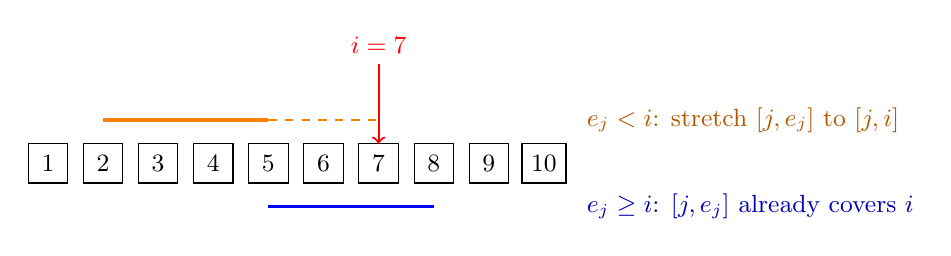
\begin{tikzpicture}[x=0.7cm,y=0.55cm]
  \foreach \x in {1,...,10} \node[draw,minimum size=0.5cm] at (\x,0) {\small\x};
  \draw[very thick,orange] (2,1) -- (5,1);
  \draw[orange,dashed,thick] (5,1) -- (7,1);
  \node[anchor=west,orange!70!black] at (10.6,1) {\small $e_j<i$: stretch $[j,e_j]$ to $[j,i]$};
  \draw[very thick,blue] (5,-1) -- (8,-1);
  \node[anchor=west,blue!70!black] at (10.6,-1) {\small $e_j\ge i$: $[j,e_j]$ already covers $i$};
  \draw[->,red,thick] (7,2.3) node[above] {\small $i=7$} -- (7,0.45);
\end{tikzpicture}
\end{center}

\subsection*{Algorithm}
\begin{algorithmic}[1]
\State compute $e_j$ by two pointers
\State $open\gets\emptyset$ (pairs $(e_j-j,j)$), $p\gets1$
\For{$i=1$ \textbf{to} $N$}
  \State \textbf{if} $e_i<\infty$: insert $(e_i-i,i)$
  \While{$p\le i$ \textbf{and} $e_p<i$} erase $(e_p-p,p)$; $p\gets p+1$ \EndWhile
  \State $best\gets\min(open)$ as window $[j,e_j]$
  \State \textbf{if} $p>1$: compare with window $[p-1,i]$ (length $i-p+1$, tie on smaller $j$)
  \State print $best$
\EndFor
\end{algorithmic}

\dryrun{Test 2: shops $\{1\},\{2,3\},\{1\}$, $M=3$. $e_1=2$, $e_2=3$,
$e_3=\infty$. $i=1$: open $=\{(1,1)\}\Rightarrow(1,2)$. $i=2$: open
$\{(1,1),(1,2)\}$, tie on length, smaller $j$ $\Rightarrow(1,2)$. $i=3$:
$e_1=2<3$ so $j=1$ leaves, $p=2$; open $\{(1,2)\}\Rightarrow[2,3]$; the
stretched candidate $[1,3]$ has length $2>1$. Output $1\,2$, $1\,2$, $2\,3$.
\checkmark}

\subsection*{C++17 implementation}
\cppfile{greedy/25_cracker_shops.cpp}

\begin{complexitybox}
\textbf{Time:} $O((N+\sum X)+N\log N)$. \textbf{Space:} $O(N+M+\sum X)$.
\end{complexitybox}

\begin{pitfallbox}
\begin{itemize}
  \item The editorial's ``corner case'': near the end every minimal window
        ends before $i$, so the answer is a \emph{stretched} window --- the
        $j=p-1$ candidate.
  \item Ties: minimise length first, then $j$.
  \item Up to $10^4$ tests: allocate per test only $O(N+M)$ memory, never
        a global array of fixed maximum size reset each time.
\end{itemize}
\end{pitfallbox}

\section{Jai Hanuman}
\label{sec:g-jai-hanuman}
\problemlink{https://www.codechef.com/problems/ACM14KG4}{CodeChef ACM14KG4}
\source{ICPC 2014--15 Kharagpur Online Re-contest (PYQ, ACM14KG4)}{Medium--Hard}

\problemstatement{$N$ people and $5N$ crackers numbered $1..5N$; person $i$
starts with crackers $3i-2,3i-1,3i$. In order $1,2,\dots,N$ each person may
make up to $3$ swaps with anyone (swaps cannot be refused, Hanuman's spare
crackers included). Everyone wants three \emph{consecutive} crackers; among
those, the least one should be $\ge P_i$ and as small as possible; if that is
impossible, the least one should be as small as possible. Everybody plays
optimally and knows everything. Print each person's least cracker.}

\begin{patternbox}
Sequential moves where the \emph{last} mover cannot be disturbed
$\Rightarrow$ \textbf{backward induction}: fix the last player's outcome,
then the second last's among what is left, and so on.
\end{patternbox}

\subsection*{Approach and intuition}

Three swaps are enough to collect any three crackers, so person $N$, who moves
last, always ends with exactly the triple they want. Person $N-1$ knows this,
so anything they take from $N$'s target set will be taken away again; their
best achievable triple is the best one \emph{avoiding} $N$'s triple. Inductively,
person $i$ gets their preferred triple among crackers not wanted by
$i+1,\dots,N$.

Implementation: a start $s$ is \emph{available} while $s,s+1,s+2$ are all
free. Keep all available starts in a \texttt{set}. For person $i$ (from $N$
down to $1$) take \texttt{lower\_bound}$(P_i)$, or the smallest start if none
exists. Taking $[s,s+2]$ kills starts $s-2,\dots,s+2$. At most $5$ starts die
per person and there are $5N-2$ initially, so a start always remains.

\subsection*{Algorithm}
\begin{algorithmic}[1]
\State $S\gets\{1,\dots,5N-2\}$
\For{$i=N$ \textbf{down to} $1$}
  \State $s\gets$ smallest element of $S$ that is $\ge P_i$, else $\min S$
  \State $ans_i\gets s$; remove $s-2..s+2$ from $S$
\EndFor
\end{algorithmic}

\dryrun{$N=2$, $P=(4,9)$, crackers $1..10$. Person~2: starts $\ge9$ need
$s\le8$, none, so $s=1$ (crackers $1,2,3$). Person~1: smallest free start $\ge4$
is $4$. Output \texttt{4 1}. With $P=(1,5)$: person~2 takes $5$, person~1 takes
$1$: \texttt{1 5}. \checkmark}

\subsection*{C++17 implementation}
\cppfile{greedy/26_jai_hanuman.cpp}

\begin{complexitybox}
\textbf{Time:} $O(N\log N)$ per test. \textbf{Space:} $O(N)$.
\end{complexitybox}

\begin{pitfallbox}
\begin{itemize}
  \item Processing people from $1$ to $N$ (forward) is the natural but
        wrong reading --- earlier players do not get to keep contested
        crackers.
  \item Consecutive means \emph{any} three consecutive numbers, not aligned
        blocks $\{3i-2,3i-1,3i\}$.
\end{itemize}
\end{pitfallbox}

\section{Break, Merge and Sort}
\label{sec:g-break-merge}
\source{ICPC 2020--21 Amritapuri Preliminary, problem 3 (PYQ)}{Medium}

\begin{reconbox}
The original statement is no longer online (it was hosted on CodeDrills, which
is offline, and the Notion archive stores only the official \emph{solution
slides}). The statement below is reconstructed from those slides. The cost
model was checked by an exhaustive Dijkstra search over all split/merge
sequences on 300 random arrays: it reproduces the editorial's formula exactly.
Verify against the original if you find it.
\end{reconbox}

\problemstatement{An array $A$ of length $n$. You may \textbf{split} an array
into two contiguous non-empty parts, paying the length of the shorter part,
and \textbf{merge} two sorted arrays into one sorted array, paying the sum of
their lengths. Starting from $A$, obtain a single sorted array with minimum
total cost.}

\begin{patternbox}
Four greedy insights from the editorial: (1) all splits can be done before
all merges; (2) cut exactly at the descents $A_i>A_{i+1}$; (3) peel the
smaller end piece each time; (4) merge the two shortest arrays (Huffman).
\end{patternbox}

\subsection*{Approach and intuition}

Cutting at every descent leaves the maximal sorted runs $r_1,\dots,r_t$;
further cuts only create more merging work.

\textbf{Splitting.} Repeatedly cut off the smaller of the two end runs. Each
cut costs at most that run's length and every run except the largest is cut
off once, so splitting costs $n-\max_i r_i$ --- and this is also a lower
bound.

\textbf{Merging.} Merging behaves like building a Huffman tree: a run merged
$c_i$ times contributes $c_i\cdot r_i$, where $c_i$ is its depth in the merge
tree. As in Huffman coding, there is an optimal tree in which the two
shortest runs are siblings, so ``always merge the two shortest'' is optimal.

\begin{center}
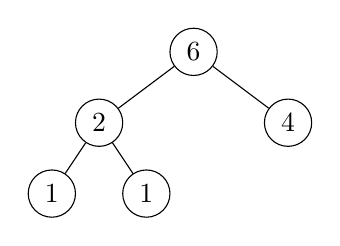
\begin{tikzpicture}[level distance=0.9cm,
  every node/.style={draw,circle,minimum size=0.6cm,inner sep=1pt},
  level 1/.style={sibling distance=2.4cm},
  level 2/.style={sibling distance=1.2cm}]
\node {6}
  child {node {2} child {node {1}} child {node {1}}}
  child {node {4}};
\end{tikzpicture}
\qquad
\begin{minipage}{6.5cm}\small
Runs $1,1,4$: merge $1+1$ (cost $2$), then $2+4$ (cost $6$): merging
cost $8$ = $\sum$ internal nodes.
\end{minipage}
\end{center}

\begin{ideabox}[Total Cost]
\[
  \text{answer}=\bigl(n-\max_i r_i\bigr)+\text{Huffman}(r_1,\dots,r_t).
\]
\end{ideabox}

\subsection*{Algorithm}
\begin{algorithmic}[1]
\State split $A$ into maximal non-decreasing runs $r_1..r_t$
\State $cost\gets n-\max r$; push all $r_i$ into a min-heap
\While{heap size $>1$} \State pop $x,y$; $cost\gets cost+x+y$; push $x+y$ \EndWhile
\State \Return $cost$
\end{algorithmic}

\dryrun{$A=[3,1,4,2]$: runs $[3],[1,4],[2]$, lengths $1,2,1$. Split cost
$4-2=2$. Huffman: $1+1=2$ (cost $2$), $2+2=4$ (cost $4$). Total $8$. A sorted
array has one run and costs $0$. \checkmark}

\subsection*{C++17 implementation}
\cppfile{greedy/27_break_merge_and_sort.cpp}

\begin{complexitybox}
\textbf{Time:} $O(n\log n)$. \textbf{Space:} $O(n)$.
\end{complexitybox}

\begin{pitfallbox}
\begin{itemize}
  \item Equal neighbours are \emph{not} a descent (non-decreasing runs).
  \item Merging runs left-to-right is the classic wrong answer: lengths
        $1,1,1,100$ merged left to right cost $2+3+103=108$; Huffman also
        gives $108$ here, but for $100,1,1,1$ left to right costs
        $101+102+103=306$ vs Huffman $2+3+103=108$.
\end{itemize}
\end{pitfallbox}

\section{Minimum Weight Bi-Partition}
\label{sec:g-min-bipartition}
\problemlink{https://github.com/m-e-r-l-i-n/icpc-india/blob/main/src/ICPC\%202020\%20-\%20India\%20Prelims\%20Solutions.pdf}{Contest PDF (official 2020 solution slides; original CodeDrills page is offline)}
\source{ICPC 2020--21 Amritapuri Preliminary, problem 4 (PYQ)}{Medium}

\begin{reconbox}
Only the official solution slides survive. They reduce the problem to: ``a
tree is a connected bipartite graph, so after adding new edges it is enough to
find an MST; sorting vertices by $A_i$ and joining consecutive ones gives the
only $n-1$ new edges that matter; existing edges have weight $0$.'' This
section solves that core task. The full original statement may add conditions
that this reduction already handles; check the original if you find it.
\end{reconbox}

\problemstatement{A graph has $n$ vertices with values $A_i$ and $m$ existing
edges, which are free. You may add an edge $(u,v)$ at cost $|A_u-A_v|$. Find
the minimum total cost to make the graph connected (equivalently, the weight
of a minimum spanning tree of the complete graph where existing edges weigh
$0$).}

\begin{patternbox}
MST on a complete graph with weights $|A_u-A_v|$ $\Rightarrow$ only
\textbf{adjacent-in-sorted-order} edges can be useful: $O(n)$ candidate edges
instead of $O(n^2)$.
\end{patternbox}

\subsection*{Approach and intuition}

Sort the vertices by value: $A_{v_1}\le\dots\le A_{v_n}$. For $i<j$ the edge
$(v_i,v_j)$ has weight $A_{v_j}-A_{v_i}$, which equals the total weight of the
path $v_i,v_{i+1},\dots,v_j$, and each edge on that path is no heavier. By the
cycle property of MSTs, a heaviest edge on a cycle is never needed, so the
long edge can be dropped. The candidate set is: the $m$ free edges plus the
$n-1$ sorted-neighbour edges. Run Kruskal with a DSU.

\subsection*{Algorithm}
\begin{algorithmic}[1]
\State $E\gets\{(0,u,v)\text{ for existing edges}\}\cup\{(A_{v_{i+1}}-A_{v_i},v_i,v_{i+1})\}$
\State sort $E$; DSU on $n$ vertices; $cost\gets0$
\For{$(w,u,v)\in E$} \If{\textsc{Unite}$(u,v)$} $cost\gets cost+w$ \EndIf \EndFor
\State \Return $cost$
\end{algorithmic}

\dryrun{$A=[5,1,9,4]$, existing edge $(1,3)$. Sorted: $v=2,4,1,3$ (values
$1,4,5,9$). Edges: $(1,3)$ free; $(2,4)=3$, $(4,1)=1$, $(1,3)=4$. Kruskal:
free $(1,3)$, then $(4,1)$ cost $1$, then $(2,4)$ cost $3$; $(1,3)$ now
redundant. Total $4$. \checkmark\ (checked against Prim on the full graph)}

\subsection*{C++17 implementation}
\cppfile{greedy/28_min_weight_bipartition.cpp}

\begin{complexitybox}
\textbf{Time:} $O((n+m)\log(n+m))$. \textbf{Space:} $O(n+m)$.
\end{complexitybox}

\begin{pitfallbox}
\begin{itemize}
  \item Building all $\binom n2$ edges is $O(n^2)$ --- TLE for $n=10^5$.
  \item Self-loops and multi-edges among the free edges are harmless in
        Kruskal.
\end{itemize}
\end{pitfallbox}

\section{Coins}
\label{sec:g-coins}
\source{AtCoder AGC018 C (Notion: Greedy, stretch goal)}{Hard}

\problemstatement{$X+Y+Z\le10^5$ people; person $i$ has $A_i$ gold, $B_i$
silver and $C_i$ bronze coins. Take gold from exactly $X$ people, silver from
$Y$ others and bronze from the remaining $Z$. Maximise the total number of
coins.}

\begin{patternbox}
Three-way assignment $\to$ subtract one option to get a two-way problem, then
an \textbf{exchange argument} shows the two groups are separated by one sort
order. Try every split point with prefix/suffix \textbf{top-$k$ heaps}.
\end{patternbox}

\subsection*{Approach and intuition}

Everyone gives bronze by default: start from $\sum C_i$ and let $a_i=A_i-C_i$,
$b_i=B_i-C_i$. Now choose $X$ people for $a$ and $Y$ other people for $b$.

\begin{ideabox}[Exchange Argument]
If $p$ is gold and $q$ is silver with $a_p-b_p<a_q-b_q$, swapping their roles
changes the total by $(a_q+b_p)-(a_p+b_q)=(a_q-b_q)-(a_p-b_p)>0$. So in an
optimal solution, after sorting by $a_i-b_i$ descending, every gold person
comes before every silver person: there is a split $k$ with gold chosen among
the first $k$ people and silver among the last $n-k$.
\end{ideabox}

For each $k$, the best gold choice is the $X$ largest $a$ in the prefix and
the best silver choice the $Y$ largest $b$ in the suffix. Both are maintained
incrementally with a min-heap of size $X$ (resp.\ $Y$).

\subsection*{Algorithm}
\begin{algorithmic}[1]
\State $base\gets\sum C_i$; sort people by $a_i-b_i$ descending
\State $L[k]\gets$ sum of $X$ largest $a$ among the first $k$ (min-heap)
\State $R[k]\gets$ sum of $Y$ largest $b$ among people $k..n-1$ (min-heap)
\State \Return $base+\max_{X\le k\le n-Y}(L[k]+R[k])$
\end{algorithmic}

\dryrun{Sample 1 ($X=1,Y=2,Z=1$): $\sum C=15$; $(a,b)=(-2,0),(2,1),(0,-1),(2,-1)$.
Sorted by $a-b$: $(2,-1),(0,-1),(2,1),(-2,0)$. At $k=1$: gold $a=2$, best two $b$
among the rest $=1+0$; total $15+3=18$. \checkmark}

\subsection*{C++17 implementation}
\cppfile{greedy/29_coins.cpp}

\begin{complexitybox}
\textbf{Time:} $O(n\log n)$. \textbf{Space:} $O(n)$.
\end{complexitybox}

\begin{pitfallbox}
\begin{itemize}
  \item Greedy ``give each person their best colour'' ignores the exact
        quotas $X,Y,Z$.
  \item Sums reach $3\cdot10^{14}$: \texttt{long long}.
\end{itemize}
\end{pitfallbox}

